\documentclass{llncs}
%
\usepackage{makeidx}  % allows for indexgeneration
\usepackage[pdftex]{hyperref}
\usepackage{graphicx}
%
\begin{document}
%
\frontmatter          % for the preliminaries
%
\pagestyle{headings}  % switches on printing of running  heads
%
%
%
\mainmatter              % start of the contributions
%
\title{
The Electrical Grid and Supercomputer Centers:  
An Investigative Analysis of Emerging Opportunities and Challenges
}

%
\titlerunning{Electrical Grid}  % abbreviated title (for running head)
% also used for the TOC unless 
% \toctitle is used
%
%
\author{Fname Lname\inst{1} \and Fname Lname\inst{2}
Fname Lname \and Fname Lname \and Fname Lname \and Fname~M.~Lname \and
Fname Lname}
%
\authorrunning{Fname Lname et al.} % abbreviated author list (for running head)
%
%
\institute{Institute Name, City State Zip, Country,\\
\email{Name@email.adr},\\ WWW home page:
\texttt{http://web/page.html}
\and
Another Institute,
nstitute Department, address1,\\
address2, Country}

\maketitle              % typeset the title of the contribution

\begin{abstract}
Some of the largest supercomputer centers in the United 
States are developing new relationships with their 
electricity providers.  These relationships are driven by 
mutual interest.  Supercomputer centers are concerned about 
electricity price, quality, environmental impact and 
availability. Electricity providers are concerned about 
supercomputer center's impact on the electrical grid, both 
for energy consumption, peak power and fluctuations in 
power. Supercomputer center power demand can be greater 
than 20 megawatts (MW), theoretical peak power requirements 
greater than 45MW and re-occurring intra-hour variability 
can exceed 8MW. As a consequence, there are some 
supercomputer centers whose electricity providers are 
asking for hourly forecasts of power demand, a day in 
advance.   This paper explores today's relationships, 
potential partnerships and possible integration between 
supercomputer centers and their electricity providers. It 
develops a model for possible integration between 
supercomputer centers and the electrical grid. It then 
explores the utility of this model based on feedback from a 
questionnaire of Top 100 List sized supercomputer centers 
in the United States.
\end{abstract}

%
\section{Introduction}
%
Supercomputer centers with petascale systems for high-performance 
computing (HPC) are realizing the large impact they will be 
putting on their electricity service providers as they bring on 
(and perhaps turnoff or idle) megawatt scale (some double digit) supercomputers.
 
The Energy Efficient HPC Working Group 
(\href {http://eehpcwg.lbl.gov/}{EE HPC WG}) 
has been investigating opportunities for large supercomputing sites to more closely 
integrate with their electricity service providers. This paper documents the 
results of this investigative activity. 

Leveraging prior work on data center and grid integration opportunities done
by Lawrence Berkeley National Laboratory's Demand Response Research Center
(\href
{http://drrc.lbl.gov/publications/demand-response-and-open-automated-demand-response-opportunities-data-centers}{http://drrc.lbl.gov/publications}),
 this paper takes as a starting point LBNL's model for integrating data
centers and the electrical grid. The model describes programs that are used
by the electricity service providers to integrate with their customers (such
as demand response) and methods used to balance the grid supply and demand
of electricity. It also describes strategies that data centers might employ
for managing their electricity and power requirements. This paper tuned this
model's data center strategies for supercomputer centers.

The first section of this paper describes in greater detail the model for
integrating supercomputer centers and the electrical grid. The second
section is a review of prior work on HPC center strategies that might be
deployed for managing electricity and power. In order to further understand
today's relationships, potential partnerships and possible integration
between HPC centers, their electricity providers and the grid, a
questionnaire was deployed whose respondents were Top100 List class
supercomputer centers in the United States. The third section of this paper
describes the results of that questionnaire. The fourth section of the paper
describes opportunities, solutions and barriers. A fifth section describes
conclusions and next steps. Finally, the last section recognizes additional

%
\section{Supercomputing Centers and Electrical Grid Integration}
%
The EE HPC WG Team took as their starting point a model developed by
Lawrence Berkeley National Laboratory's Demand Reponse Research Center
\href{http://drrc.lbl.gov/publications/demand-response-and-open-automated-demand-response-opportunities-data-centers}
{http://drrc.lbl.gov/publications}
 that describes ways in which data centers and electricity service
providers may interact. This model describes programs that are used by the
electricity service providers to encourage particular behaviors by their
customers and methods used to balance the grid supply and demand of
electricity. It also describes strategies that data centers might employ for
managing their electricity and power requirements. The EE HPC WG Team
adopted this model with slight tweaks to reflect the HPC environment (versus
the general data center).

\subsection{Electricity Provider Programs and Methods}
Programs are used by the electricity service providers to encourage
particular behaviors by their customers. Methods used to balance the grid
supply and demand of electricity.

Below is a list of programs and methods:


\begin{itemize}
\item Energy Efficiency: Programs used to reduce overall electricity consumption, generally but not always at times of
 peak demand.
\item Peak Shaving (shed): Programs used to reduce load during peak times, where the reduced load is not used at a 
later time.
\item Peak Shaving (shift): Programs where the load during peak times is moved to, typically, non-peak hours.
\item Dynamic Pricing: Time varying pricing programs used to increase, shed or shift electricity consumption.
\item Grid Scale Storage: Methods used to store electricity on a large scale. Pumped-storage hydroelectricity 
is the largest-capacity form of grid energy storage.
\item Renewable (off-site): Methods used to manage the variable uncertain generation nature of many renewable resources.
\item Frequency response: Methods used to keep grid frequency constant and in-balance. Generators are typically used for frequency response.
\item Regulation (Up or Down): Methods used to maintain that portion of electricity generation reserves 
that are needed to balance generation and demand at all times.
\item Congestion: Methods used to resolve congestion that occurs when there is not enough transmission capability to 
support all requests for transmission services. Or, methods used to resolve congestion that occurs when the distributio
\end{itemize}

\subsection{Supercomputer Center Strageties}

Another dimension of the model is a list of strategies that a supercomputer
site might use for managing power in response to a request from their
electric service provider.

Although these strategies can be used for managing power in response to a
request from an electric service provider, many of them could also be used
for improving energy efficiency. It is the former that is of primary
interest to this investigation. Two examples may help to clarify this
distinction. Load migration is an example of a strategy that is well suited
to responding to an electric service provider request, but is not likely to
improve energy efficiency. Fine grained power management, on the other hand,
is more likely to be used for improving energy efficiency than for
responding to electric service provider requests.

Below is a list of strategies:

\begin{itemize}
\item Fine grained power management refers to the ability to control HPC system power 
and energy with tools that are high resolution control and can target specific 
low level sub-systems. A typical example is voltage and frequency scaling of the CPU.

\item Course grained power management also refers to the ability to control HPC 
system power and energy, but contrasts with fine grained power management in 
that the resolution is low and it is generally done at a more aggregated level. 
A typical example is power capping.

\item Load migration refers to temporarily shifting computing loads from 
an HPC system in one site to a system in another location.

\item Job scheduling refers to the ability to control HPC system power 
by understanding the power profile of applications and queuing the 
applications based on those profiles.

\item Back-up scheduling refers to deferring data storage processes to off-peak periods.

\item Shutdown refers to a graceful shutdown of idle HPC equipment. It usually 
applies when there is redundancy.

\item Lighting control allows for data center lights to be shutdown completely.

\item Thermal management is widening temperature set-point ranges and 
humidity levels for short periods.
\end{itemize}

\section{Prior Work}

The prior work described in this paper is that which addresses strategies
that HPC centers can take to manage power. A lot of work has been done on
energy efficiency, some of which has an element of power management. But,
there is not a lot work that is specifically focused on power management in
response to a request from an electrical service provider.

\subsection{Fine Grained Power Management}
In \cite{varma_control-theoretic_2003} (Varma et al., 2003) system level DVFS techniques demonstrated. They
monitor CPU utilization at regular intervals and then perform dynamic
scaling based on their estimate of utilization for the next interval.

Authors in\cite{von_laszewski_power-aware_2009} (von Laszewski et al., 2009) present an efficient scheduling
algorithm to allocate virtual machines in a DVFS-enabled cluster by
dynamically scaling the supplied voltages.

vGreen \cite{dhiman_vgreen:_2009} (Dhiman et al., 2009) is a system for energy efficient computing in
virtualized environments by linking online workload characterization to
dynamic VM scheduling decisions to achieve better performance, energy
efficiency and power balance in the system.

\subsection{Power Capping}

\textbf{Power capping }techniques set a value below the actual peak power
and preventing that number from being exceeded through some type of control
loop [Fan07]. There are numerous ways to implement this, but they generally
consist of a \textbf{power monitoring system }such as a power estimation
method or one based on direct power sensing, and a \textbf{power throttling
mechanism}. Power throttling generally works best when there is \textbf{a
set of jobs with loose service level guarantees or low priority }that can be
forced to reduce consumption when the data center is approaching \textbf{the
power cap value}. Power consumption can be reduced simply by
\textbf{de-scheduling tasks }or by using any available component-level power
management \textbf{knobs}, such as DVFS [Fan07]
.

\subsection{Job Scheduling}
The problem of scheduling jobs has been extensively studied. In general,
most of the schedulers implement the First Come First Served (FCFS) policy
as a simple but fair strategy for scheduling jobs. But this policy suffers
from low system utilization. The most commonly used optimization is backfill
\cite{lifka_anl/ibm_1995} 
\cite{mualem_utilization_2001}
\cite{feitelson_parallel_2004}
[Lif95, Mua95, Fei04]. Backfilling is proposed to improve the system
utilization. Backfilling by identifying free capacities allows the smaller
jobs fit those capacities to move forward and run on idle processors.

In 
[Yang ref is not in Zotero] 
\cite{zhou_reducing_2013}
[Yang13] and [Zhou13] , \textbf{job scheduling} as a DR strategy and
\textbf{dynamic pricing} as a grid integration program have been used to
propose \textbf{a power-aware job scheduling} approach to reduce
\textbf{electricity costs} \textit{without degrading the system utilization}. 
The novelty of the proposed job scheduling
mechanism is its ability to take \textit{the variation of 
electricity price }into consideration as a means to make
better decisions of the timing of scheduling jobs with diverse power
profiles. Experimentations on an IBM Blue Gene/P and a cluster system as
well as a case study on Argonne's 48-rack IBM Blue Gene/Q system have
demonstrated the effectiveness of this scheduling approach. Preliminary
results show a \textbf{23{\%}} reduction in electricity cost of HPC systems.

A grid computing infrastructure with large amount of computations normally
contains parallel machines (supercomputers cluster) as main computational
resources 
\cite{foster_anatomy_2001} [Fos01]
. Incoming jobs to Grid's local resources are scheduled by
local scheduling system. Local scheduling system for parallel machines
typically use batch queued space-sharing and its variants as scheduling
policies. Most current local schedulers use backfilling strategies with FCFS
queue-priority order as policy for parallel job scheduling. In the US,
supercomputer centers are connected via grid computing infrastructures such
as TeraGrid, Open Science Grid. Grid computing's protocols, interfaces, and
standards can facilitate the execution of DR strategies, as a result grid
computing may increase the interest level and/or the impact level of DR
strategies.

There are many use cases in grid computing environment that require QoS
guarantees in terms of guaranteed response time, including time-critical
tasks that must meet a deadline, which would be impossible without a start
time guarantee. Furthermore providing time guarantee enable the job to be
coordinated with other activities, essential for co-allocation and workflows
applications. Advance reservation is a guarantee for the availability of a
certain amount of resources to users and applications at specific times in
the future 
\cite{foster_distributed_1999} [Fos99]. Advance reservation feature requires local scheduling
systems to support a reservation capability beside batch queued policy for
local and normal jobs. In load migration, we encounter the need to deliver
resources at specific times in order to accept jobs from other HPC centers
to respond to their demand enforced by electricity grid. This requirement
can be achieved by advance reservations 
\cite{foster_distributed_1999}
[Fos99]. Modern resource management
and scheduling systems such as Sun Grid Engine, PBS, OpenPBS, Torque, Maui,
and Moab support backfilling and advance reservation capabilities.

By using \textit{advance reservation capabilities }of schedulers 
(within local resource managers) of HPC centers, we
facilitate \textit{the execution of load migration strategy }between 
HPC centers (e.g., in terms of automation); as a result
we increase the interest level and to some extent the impact level of load
migration strategies.

\subsection{Load Migration}

In order to balance the electrical grid,
\cite{chiu_electric_2012}
[Chiu12] proposes a low-cost
\textbf{geographic load migration} to match electricity supply. In addition,
authors present a real grid balancing problem experienced in the Pacific
Northwest. They propose a symbiotic relationship between data centers and
electrical grid operators by showing that \textbf{mutual cost benefits }can
be accessible.

\subsection{Thermal Management}
Thermal and cooling metrics are becoming important metrics in scheduling and
resource management of HPC centers. Runtime cooling strategies are mostly
job-placement-centric. These techniques either aim to place incoming
computationally intensive jobs in a thermal-aware manner on servers with
lower temperatures or attempt to reactively migrate/load-balance jobs from
high temperature servers to servers with lower temperatures.
\textbf{\textit{T* }} 

\cite{kaushik_t*:_2012}
[Kau12]
 takes a data-centric thermal- and
energy-management approach and does proactive, thermal-aware file placement
which allows cooling energy costs savings without performance trade-offs. T*
is cognizant of the uneven thermal-profile of the servers, differences in
their thermal-reliability-driven load thresholds, and differences in the
data-semantics, i.e., computation job rates, sizes, and evolution life
spans, of the big data placed in the cluster.

In this paper, we assume that the grid is a given constant as a fundamental
property. But, grid integration solutions may take into consideration that
it isn't a given as electrical grid infrastructures will evolve in the
future 
\cite{he_architecture_2008}
[He08]
. Thus, changes in the grid could make grid integration more or
less difficult.

In 
\cite{aikema_electrical_2011}
[Aik11] , authors explored the potential for HPC centers to adapt to
dynamic electrical prices, variation in carbon intensity within an
electrical grid, or availability of local renewables. Through simulations
experiments on workloads from the Parallel Workloads Archive alongside
real-world pricing data, they demonstrate potential savings on the cost of
electricity ranging typically between 10-50{\%}. Nonetheless, adaptation to
the variation in the electrical grid carbon intensity was not as successful,
but adaptation to the availability of local renewables showed potential to
significantly increase their use.

\section{Questionaire} 
We used a questionnaire in order to understand the current experiences of
supercomputer centers with respect to interacting with their electricity
service providers. We restricted the analysis to sites in the United States
since the results of the survey and practices of demand response is highly
correlated and driven by energy policies in the country. 
\cite{torriti_demand_2010}
[Tor10].

Nineteen Top100 List sized sites in the United States were targeted for the
questionnaire. Eleven sites responded (ORNL, LLNL, ANL, LANL, LBNL, WPAFB,
NOAA, NCSA, SDSC, Purdue, and Intel) and eight sites didn't respond (NCAR,
IBM, NETL, Indiana University, TACC, SNL, NREL, NASA). The questionnaire was
sent to a sample that was not randomly selected. It was sent to those sites
where it was relatively easy to identify an individual based on membership
within the EE HPC WG. The sample is more representative of Top50 sized sites
(1 Top50 sized site was not in the sample and 60{\%} (9/15) of the sample
responded). Only 4 additional sites were sampled from the Top51-Top100 List
and, of those, 2 responded (Intel and NOAA).

The total power load as well as the intra-hour fluctuation of these sites
varied significantly. There were four sites with total power load greater
than 10MW, two sites with \textasciitilde 5MW total power load and five
sites with less than 2MW total power load. We chose less than 3MW intra hour
variability as the bottom of the scale because we assumed that the
electrical service providers would not be affected by that magnitude of
fluctuation. For those with total power load greater than 10MW, the
intra-hour fluctuation varied from less than 3MW to 8MW. One of
\textasciitilde 5MW sites said that they experienced 4MW variability. The
rest of the sites were all less than 3MW. Most of the intra-hour variability
was due to preventative maintenance.





\begin{table}[htbp]

\begin{center}
\caption{Caption Number 1}
\begin{tabular}{|p{65pt}|l|l|}
\hline
\textbf{Total Load}&
\textbf{Variability}&
\textbf{Frequency} \\
\hline
16-17MW&
5MW&
weekly \\
\hline
13-14MW&
8MW&
monthly \\
\hline
10-11MW&
Less than 3MW&
weekly \\
\hline
10-11MW&
7MW&
weekly \\
\hline
4-5MW&
Less than 3MW&
weekly \\
\hline
4-5MW&
4MW&
weekly \\
\hline
1-2MW&
Less than 3MW&
weekly \\
\hline
1-2MW&
140kW&
daily \\
\hline
1-2MW&
Less than 3MW&
yearly \\
\hline
1-2MW&
200kW or less&
daily \\
\hline
1-2MW&
Less than 3MW&
daily \\
\hline
\end{tabular}
\label{tab1}
\end{center}
\end{table}

We asked if the supercomputer centers had talked to their electric service
providers about programs and methods used to balance the grid supply and
demand of electricity. About half of them have had some discussion, but it
has mostly been limited to programs and not methods.

\begin{table}[htbp]

\begin{center}
\caption{Caption Number 2}
\begin{tabular}{|p{230pt}|l|}
\hline
\textbf{Discussions with Electricity Providers}&
{\%} Answered Yes \\
\hline
\textbf{Programs}&
~ \\
\hline
Shedding load during peak demand&
54 \\
\hline
Responding to pricing incentive programs&
45 \\
\hline
Shifting load during peak demand&
36 \\
\hline
\textbf{Methods}&
~ \\
\hline
Enabling use of renewables&
36 \\
\hline
Congestion, Regulation, Frequency Response&
18 \\
\hline
Contributing to electrical grid storage&
10 \\
\hline
\end{tabular}
\label{tab2}
\end{center}
\end{table}


More than half of the respondents are not interested in shedding or shifting
load during peak demand. There is some indication that this low interest is
primarily due to the lack of a clear business case. For the sites where
there is interest, shifting is more attractive than shedding load. SDSC is
an exception to this trend, but because of a site-wide program. ``UCSD
generates 30-35MW of power yet still imports 5-10MW. As a large generation
source the utility providers see the campus as a highly attractive partner
for offloading grid stress. Automatic load shedding is being
explored/deployed today.''

Responding to pricing incentive programs is also not considered interesting,
although the reasons for this low interest may be organizational. Several
open-ended comments revealed that pricing is fixed and/or done by another
organization at the site level and outside of their immediate control.

Eighty percent of the respondents have not had discussions with their
electricity service providers about congestion, regulation and frequency
response. LANL is one of two who have had discussions and who commented that
they are ``learning about the process'' and that it is ``outside of [their]

visibility or control''.

There were been many more respondents who have had discussions with their
electricity service providers about enabling the use of renewables; 36{\%}
have already had discussions and more than half are interested in further
and/or future discussions. SDSC already has a site-wide program; ``the
campus has a large fuel cell (2.5$+$ MW) and works with the utility with
renewables.'' Other responses suggest that the interest is at the site level
and not unique to the supercomputer center.

An open-ended question was posed as to whether or not there was information
either requested of the supercomputer sites by their providers or,
conversely, requested of the providers by the sites. In both cases, well
over 75{\%} of the respondents answered no. LLNL and LANL were the
exceptions. LLNL is ``working on obtaining additional data from them and a
means of sharing data between them and us'' and has been requested to
provide ``additional detailed forecasting and ultimately real time data.''
LANL has also been requested to provide ``power projections, hour by hour,
for at least a day in advance'' and, perhaps as a consequence, would like to
have more information on ``sensitivity of power distribution grid to rapid
transients (random daily step changes of 10 MW up or down within a single AC
cycle).''

Given the low levels of current engagement between the electricity service
providers and the supercomputer centers, it is not surprising that none of
the supercomputer centers are currently using any power management
strategies to respond to grid requests by their electrical service
providers. SDSC's \textit{supercomputer center} is not an exception, but they did respond that their
entire ``campus is leveraging parallel electrical distribution to trigger
diesel generators and other back-up resources to respond to to grid and
non-grid requests.''

We tried to evaluate if power management strategies will be considered
relevant and effective for grid integration at some point in the future. Two
questions were asked; is there interest in using the strategies and what
impact did they think that the strategies would have. When combining
interest and impact, the results showed that power capping, shutdown, and
job scheduling were both high interest and impact. Load migration, back-up
scheduling, fine grained power management and thermal management were medium
interest and impact. Lighting control and back-up resources were low
interest and impact.


\begin{table}[htbp]

\begin{center}
\caption{Caption Number 3}
\begin{tabular}{|p{299pt}|}
\hline
\textbf{HPC strategies for responding to Electricity Provider requests (listed from highest to lowest interest }$+$\textbf{ impact)} \\
\hline
Course grained power management \\
\hline
Facility shutdown \\
\hline
Job scheduling \\
\hline
Load migration \\
\hline
Re-scheduling back-ups \\
\hline
Fine grained power management \\
\hline
Temperature control beyond ASHRAE limits \\
\hline
Turn off lighting \\
\hline
Use back-up resources (e.g., generators) \\
\hline
\end{tabular}
\label{tab3}
\end{center}
\end{table}



\section{Opportunities/Solutions and Barriers} 

[koenig -- 01-NOV-2013] These are things I think this section should
include:

\begin{enumerate}
\item Link the beginning of this section to the end of the previous (Survey Results) section by suggesting that the biggest ``opportuni
ty'' is to start a process of negotiation/interaction between utility providers and HPC centers; the survey data seems to indicate that
 this is being asked for by providers, at least in some small way already
\item opportunities related to system software
        \begin{itemize}
        \item If negotiation starts happening between utility providers and HPC center operators, the system software (i.e., job schedu
ler) is a key component in order to ensure that this happens as efficiently as possible in order to keep high utilization / business ut
ility going at the HPC center (consider here things such as fluctuations in HPC use; e.g., things like large-scale acceptance / Top500
style runs)
        \item just lowering the power consumption of a batch job (i.e., by using fine grained power management techniques) does not ens
ure that the overall energy consumption is reduced; need some kind of knowledge about the workflow in the organization to make these ki
nds of determinations
        \item in addition to the advanced reservation capabilities discussed in the three paragraphs above, other areas where system so
ftware can participate are
                \begin{itemize}
                \item power capping
                \item temperature adjustment within the datacenter (make reference to discussion on Page 6)
                \item load migration - requires cooperation by HPC centers; also, migrating large datasets is hard
                \end{itemize}
        \item need to expose ``knobs'' into the system software so that HPC facility managers can easily adjust the objectives that the
 system software is using to make decisions because the overall number of ways of scheduling a workflow makes the problem too hard to r
eadily solve by hand
        \end{itemize}
\item if there is some kind of automated ``negotiation'' process that takes place between utility providers and HPC centers, it's likel
y that the utility providers will need to improve their capabilities to be able to participate in this process (e.g., probably need to
solve some kind of weighted optimization problem in near real time in order to know where the most important places are to ensure unint
errupted service); there is an opportunity to the utility provider in this, however, in that these advancements in their technology for
 monitoring and adjusting their infrastructure might be leveraged toward other ends that are not related to HPC centers specifically
\end{enumerate}


\section{Conclusions and Next Steps}

\begin{enumerate}
\item Potential HPC-specific value proposition for active DR engagement
\item Based on Grid Integration solutions -- local and system-wide impacts
\item Next steps -- specific directions or target areas to focus
\end{enumerate}

Electricity providers have viewed the hourly, daily, and seasonal
fluctuations of demand as facts of life. These fluctuations required
additional generating capacity, particularly peaking plants that were needed
only a few hours per year.

DR adoption: automation

automation technologies

DR market:

value proposition,

the measurement and verification models,

patents,

intellectual property

lighting, and heating, ventilation, and air conditioning (HVAC)

electricity-price markets

interoperability

The grid integration need to be standardized and provide interoperable
interfaces to be interoperable. Interfaces, communication infrastructure,
data, information exchange, agreement should be based on standards.
Communication with grid providers need to be standardized. grid
request/response messages. Requests include DR event, price, renewable
generation

How is architected an accounting system (energy and utilization) of an HPC
center? based on sensor systems like in [Hay09] . Sensor systems for an HPC
center to report real time power consumption of various components such as
cooling, compute systems, storage, networks, racks, etc.

[Hay09] S. Hay and A. Rice, ``The case for apportionment,'' in Proceedings
of the First ACM Workshop on Embedded Sensing Systems for Energy-Efficiency
in Buildings, New York, NY, USA, 2009, pp. 13--18.

Apportioning the total energy consumption of a building or organisation to
individual users may provide incentives to make reductions. We explore how
sensor systems installed in many buildings today can be used to apportion
energy consumption between users. We investigate the differences between a
number of possible policies to evaluate the case for apportionment based on
energy and usage data collected over the course of a year. We also study the
additional possibilities offered by more fine-grained data with reference to
case studies for specific shared resources, and discuss the potential and
challenges for future sensor systems in this area.

\begin{itemize}
\item If accounting data can be used to forecast and model future energy usage of an HPC center? so this can be communicated and be in
egrated with electricity grid.
\item If/how electricity grid providers can use energy and usage accounting data to plan electricity provisioning of an HPC center?
\item user-specific accounting data versus workload-specific accounting data.
\item accounting data in terms of HPC center components, cooling, systems, lighting, etc.
\end{itemize}
These are excellent questions. What you've outlined below is a set of value
of real-time data (the term "accounting" confused me earlier) of energy and
utilization for HPC systems. Some of these values are for EE and the rest is
how the electric grid service providers can benefit from it. For example,
telemetry data for wholesale DR markets and M{\&}V.

M{\&}V or Measurement and Verification refers to quantification of load shed
that a particular load is participating in. Typically, there are many
baseline methodologies that the utilities and ISOs use to calculate the
amount of DR a particular load/facility is providing through real-time and
day-ahead metered data. The metering and telemetry to provide the M{\&}V is
key in determining if a particular resource can participate in a DR market

and validate its performance for settlement (economics).

\newpage



%

%
% ---- Bibliography ----
%
\bibliographystyle{abbrv}
\bibliography{whitepaper}  % eehpcmethod.bib is the name of the Bibliography in this case
%

\section{Appendices}

\subsection{Background}

Over the last few years, load growth, increases in intermittent generation,
declining technology costs and increasing recognition of the importance of
customer behaviour in energy markets have brought about a change in the
focus of DR in Europe [Tor10]. The long standing programmes involving large
industries, through interruptible tariffs and time of day pricing, have been
increasingly complemented by programmes aimed at commercial and residential
customer groups.

\cite{torriti_demand_2010} Tor10] examines experiences within European countries as well as at
European Union (EU) level. While business programmes, technical and economic
potentials vary across Europe, there are common reasons as to why
coordinated DR policies have been slow to emerge: the limited knowledge on
DR energy saving capacities; high cost estimates for DR technologies and
infrastructures; and policies focused on creating the conditions for
liberalising the EU energy markets.


advances in DR It describes initiatives, studies and policies of various
European countries, with in-depth case studies of the UK, Italy and Spain.

Spees, K., {\&} Lave, L. B. (2007). Demand Response and Electricity Market
Efficiency. \textit{The Electricity Journal}, \textit{20}(3), 69--85. doi:10.1016/j.tej.2007.01.006

Interruptible Programmes represent 6.5{\%} of peak power and Load Shedding
Programmes initiate automatic load shedding in emergency situations [30].
With Interruptible Programmes participants are required to reduce their load
to predefined values. With Load Shedding Programmes utilities have the
possibility to remotely shutdown participants' equipment at short notice.
One significant difference between these two programmes is that for
Interruptible Programmes participants who do not respond can face penalties.

Load Shedding Programmes are divided into real time programmes (without
notice) and 15 min notice programmes. The size ranges from 1200 MW for real
time programmes to 1750 MW for notice programmes. Participants in these
programmes have to install and maintain Load Shedding Peripheral Units and
will be compensated according to a non-market price defined in regulation.
The size of curtailable power is of 10 MW for programmes without notice and
3 MW for programmes with notice.

Load forecasting is very important for power system operation and planning.
Traditional load forecasting tools have limitations to reflect DR customer
behaviors into load predictions. In [Zhou12], existing DR contracts are
reviewed for both wholesale and retail markets. In this study, an
illustrative example is provided to explore the impact of these contracts on
load forecasting. In conclusion, a concept of proactive load forecasting
based on contract types is proposed for forecasting loads in a smart grid
environment.

Modern hardware components such as processor, memory, disk and network offer
feature sets (Burd and Brodersen, 1995) to support energy aware operations.
Exploiting these feature sets in order to be more energy efficient is a very
important and challenging task in modeling cost/performance trade-offs, in
designing algorithms, and in defining policies. Today processors offer two
power-aware features, i.e., cpuidle and Dynamic Voltage and Frequency
Scaling (DVFS). The cpuidle feature offers a number of CPU power states
(C-states) in which they could reduce power when CPU is idle by closing some
internal gates. The CPU C-states are C0, C1, ..., Cn. C0 is the normal
working state where CPU will execute instruction, and C1, ...,Cn are
sleeping state where CPU stops executing instruction and power down some
internal components to save power. The DVFS is another power-saving method
especially when CPUs are in load line, allowing quick adjustment to
frequency/voltage upon demand in small interval. The key idea behind DVFS
techniques is to dynamically scale the supply voltage level of the CPU so as
to provide just-enough circuit speed to process the system workload, thereby
reducing the energy consumption.

We received eleven responses from the following sites: LLNL, ANL, Intel,
SDSC, Illinois, NOAA, ORNL, Purdue, AF, NERSC, LANL. The table below shows
the ranks of the responding organization in the top 100 list. 80{\%} of the
top 10, 60{\%} of the top 50, and 30{\%} of the top 100 participated in the
survey.

\begin{table}[htbp]
\begin{center}
\caption{Participating organizations and their rank in the top 100.}
\begin{tabular}{|p{59pt}|l|l|l|l|l|l|l|l|l|l|l|}
\hline
Organization&
ORNL&
LLNL&
ANL&
LANL&
NERSC&
Purdue&
AF&
NOAA&
Intel&
SDSC&
Illinois \\
\hline
Rank&
2&
3&
5&
22&
24&
28&
40&
48&
71&
102&
 \\
\hline
\end{tabular}
\label{tab4}
\end{center}
\end{table}

The survey had a total of 29 questions, eight of the questions were skipped
16 times by the 11 participants. This is only 5{\%} of the total questions
answered by the eleven participants. The graph below shows the distribution
of skipped questions.


\begin{figure}
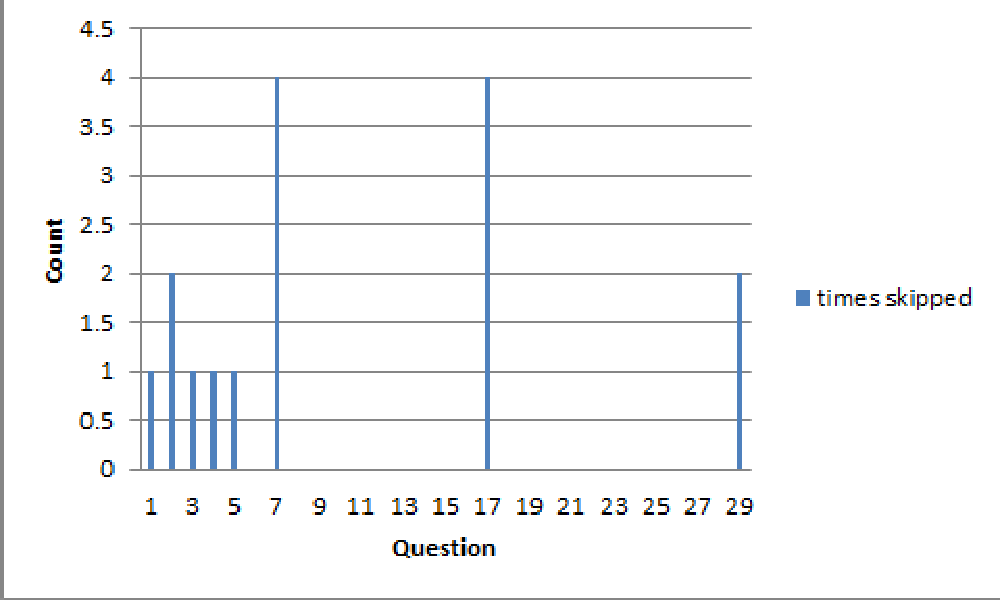
\includegraphics[width=4.01in,height=2.01in]{figure2}
\caption{Figure 2}
\end{figure}


Question 7 and 17 were skipped 4 times each, these two questions are follow
up questions to questions 6 and 16 and we were trying to collect more
details about user's responses in questions 6 and 16.

\end{document}
